\section{Experiment on a opening bottle cap task}
\label{cha4:sec3}

In the previous section we described the details of our multiple
module approach to manipulation task learning in a generic way. In this section,
we explain the experimental details for our application in the
bottle-opening task.  We demonstrate that the multiple module approach
is able to acquire human adaptive control policy and enable the robot
to master this manipulation task.

The proposed multiple module approach is implemented on a real robot system
--- the 7 DOF Light Weight KUKA robot arm\footnote{http://www.kuka-labs.com/en/medical\_robotics/lightweight\_robotics} and the 4 DOF Barrett Hand\footnote{http://www.barrett.com/robot/products-hand.htm}
for a particular manipulation task: opening bottle caps. The target of
this task is to unscrew a tightened cap until it can be lifted from
the bottle. This task is chosen as it is a common task in human daily
life, and at the same time a
complex task from the control point of view. The friction between the
bottle and the cap plays an important role in the task: it largely
determines the exerted torque required to open the cap. However, the
friction, and the way it changes as the cap unscrews, varies
between different bottles.


Estimating the friction coefficient (FCO) solely according to the
material is difficult, as it is affected by many factors such as the
load force, movement velocity, contact surface situation, composition
of the material, temperature and
etc.~\citep{gustafssoninvestigation}. A deterministic control strategy
based on the value of FCO is not practical in this task. A small
estimation error in the FCO may produce either too small torque,
which leads to task failure, or too large torque, which may cause
hardware damage. Therefore an adaptive control strategy is desired for
this
task.
We use our multiple module approach to model the adaptive strategy.

%% Why others only in simulation? what can't be simulated? [sethu2005]



\subsection{Human demonstration and experimental setup}
\label{cha4:sec3:experimentsetup}

%\begin{itemize}
%\item Dry friction can induce several types of instabilities in mechanical systems which display a stable behavior in the absence of friction.
%\item For instance, friction-related dynamical instabilities are thought to be responsible for brake squeal and the 'song' of a glass harp,[33][34] phenomena which involve stick and slip, modeled as a drop of friction coefficient with velocity.[35]
%\item Lubricated friction/dry friction
%\item not always follow Coulomb's law
%\item extremely complicated physical interaction
%\item adhesive
%\end{itemize}

% What does human do --
Opening a bottle cap is a common task for human but not an easy one
for robot. Before the task begins, the human does not possess any
information about the tightness of the cap. This information can only
be estimated once the task is started. During the task, a human will
constantly update the motor commands, i.e. how much torque to apply to
the cap and with how much force to grip the cap, according to the
sensory feedback. This plan can only be made in real time as the
contact surface condition changes along the task process. Humans have
to cope with these uncertainties and adapt to the
changes. Figure~\ref{fig:bottlepatterns} shows three different
patterns of human control strategies for three different
contexts. This task requires an adaptive strategy that controls the
turning torque, gripping force and the displacement of the
cap. Learning from human demonstration allows us to gain such a
control strategy without fully analyzing the dynamics of the whole
system..

In each demonstration, data from first time a finger touches the cap
to when the cap is finally open and lifted was recorded. Opening a
bottle cap is a cyclic task. Each cycle includes three stages:
reaching, turning and releasing. In our experiments, four to six
cycles need to be completed to open the bottles. During the reaching
and releasing stages, neither torque nor gripping force is applied to the
cap and the cap remains still. During the turning stages, humans
continuously apply torque to the cap and it starts moving once the
friction is overcome.

\begin{figure}
  \centering
  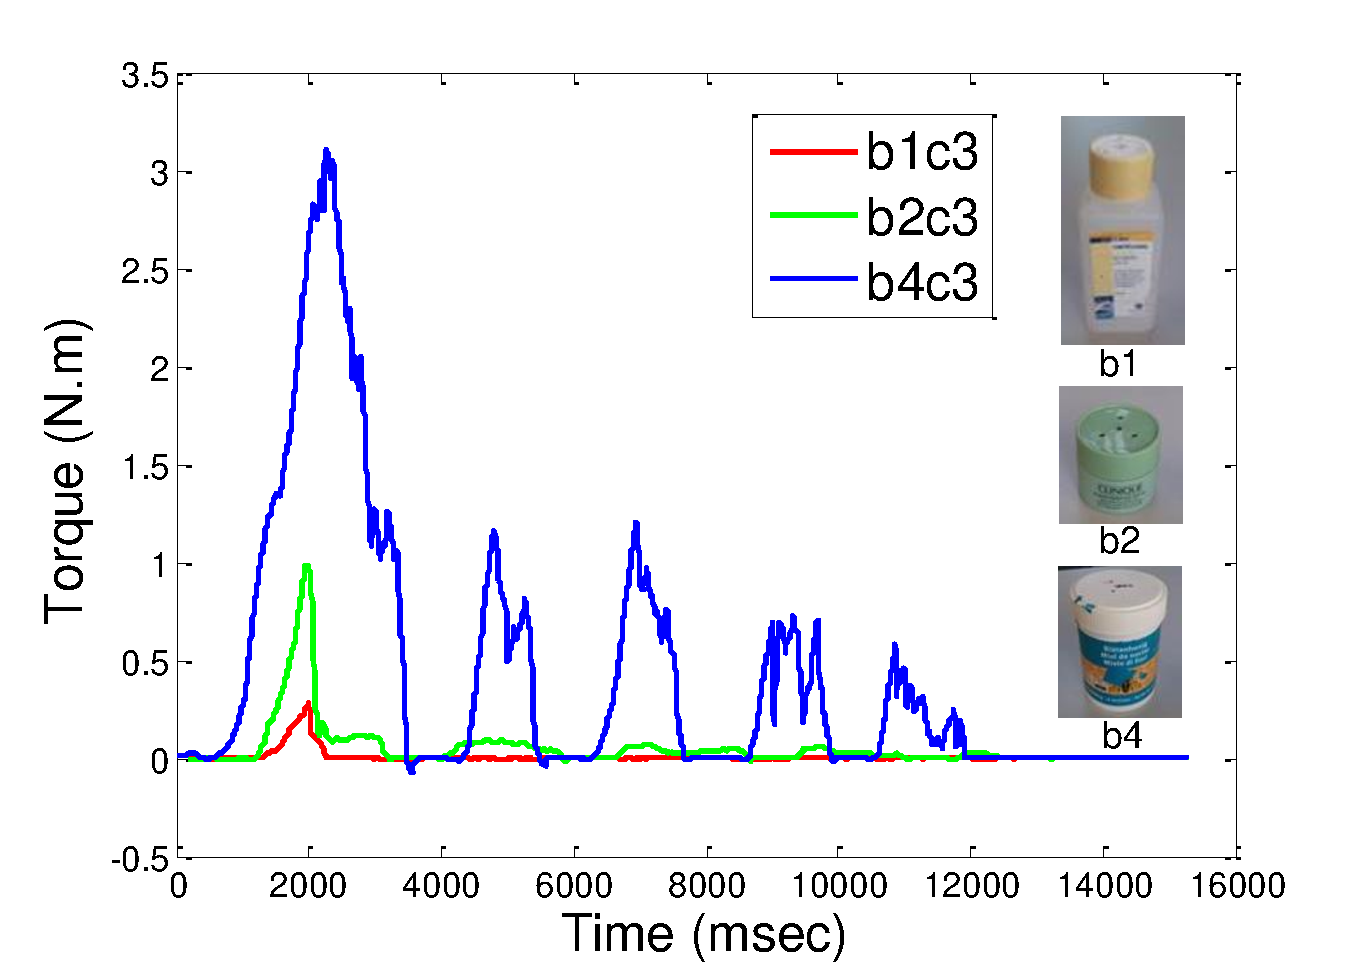
\includegraphics[width=12cm]{./fig_cha4/b1b2b4_time_T.pdf}
  \caption{ \scriptsize{Exerted torque for opening three different bottles.}
}
\label{fig:bottlepatterns}
\end{figure}


\subsubsection{Demonstration in different task contexts}
\label{cha4:sec3:experimentsetup:taskcontexts}
The experiment starts with human demonstration. In order to explore
different task contexts, we demonstrated the task with different
setups, which are the combination of four different plastic
bottles~($b1-b4$) and four different plastic caps~($c1-c4$)
(Figure.~\ref{fig:b_c}). According to the surfaces condition of the
bottles and the caps, the difficulty of opening the bottles
varies. $b1-b4$ are labeled by increasing difficulty. The bottle $b1$
is the easiest one, which originally contained body lotion. We
lubricated bottle $b1$ with its body lotion to make it even easier. The
bottle $b4$ is the most difficult one; it originally contains honey
which is very sticky. We left honey on the surfaces of $b4$ to make
it more difficult. The difficulty is estimated qualitatively. It is
judged according to the friction coefficient between the contact
surfaces. Generally speaking, the friction coefficient between
lubricated surfaces is smaller than between dry surfaces, while
between smooth surfaces is smaller than between sticky
surfaces~\footnote{Precise value of friction coefficient between
plastics varies by type of the plastic. According to an Internet
resource~\citep{FOC}, the dry dynamic friction coefficient between
plastic-plastic surface is 0.2-0.4 and the lubricated dynamic
friction coefficient is 0.04-0.1.}. The $c1-c4$ are labeled by the increasing diameters of the caps.

We chose to vary the setups in surface condition and cap size as these
are the main points of variation between the different bottles
affecting the control strategy. The intention is to see how these two
variables affect human behaviour. To this end, we combine the bottles
and the caps by mounting the caps $c1-c4$ onto the `actual'
(manufactured) caps of the bottles (Figure.~\ref{fig:setup}). To
investigate the effects of different caps and different bottles
separately, we conducted two groups of demonstrations: a fixed bottle with
four different caps ($b3c1, b3c2, b3c3, b3c4$) and a fixed cap with four
different bottles ($b1c3, b2c3, b3c3, b4c3$). Demonstrations on the
first group allow us to explore human grasping strategies with
different cap sizes. Demonstrations on the second group allow us to
explore human control strategies in adapting to different bottle
conditions. In total, we have seven different setups for the human
demonstration (Table~\ref{bottlesandcaps}).


\begin{figure}
  \centering
  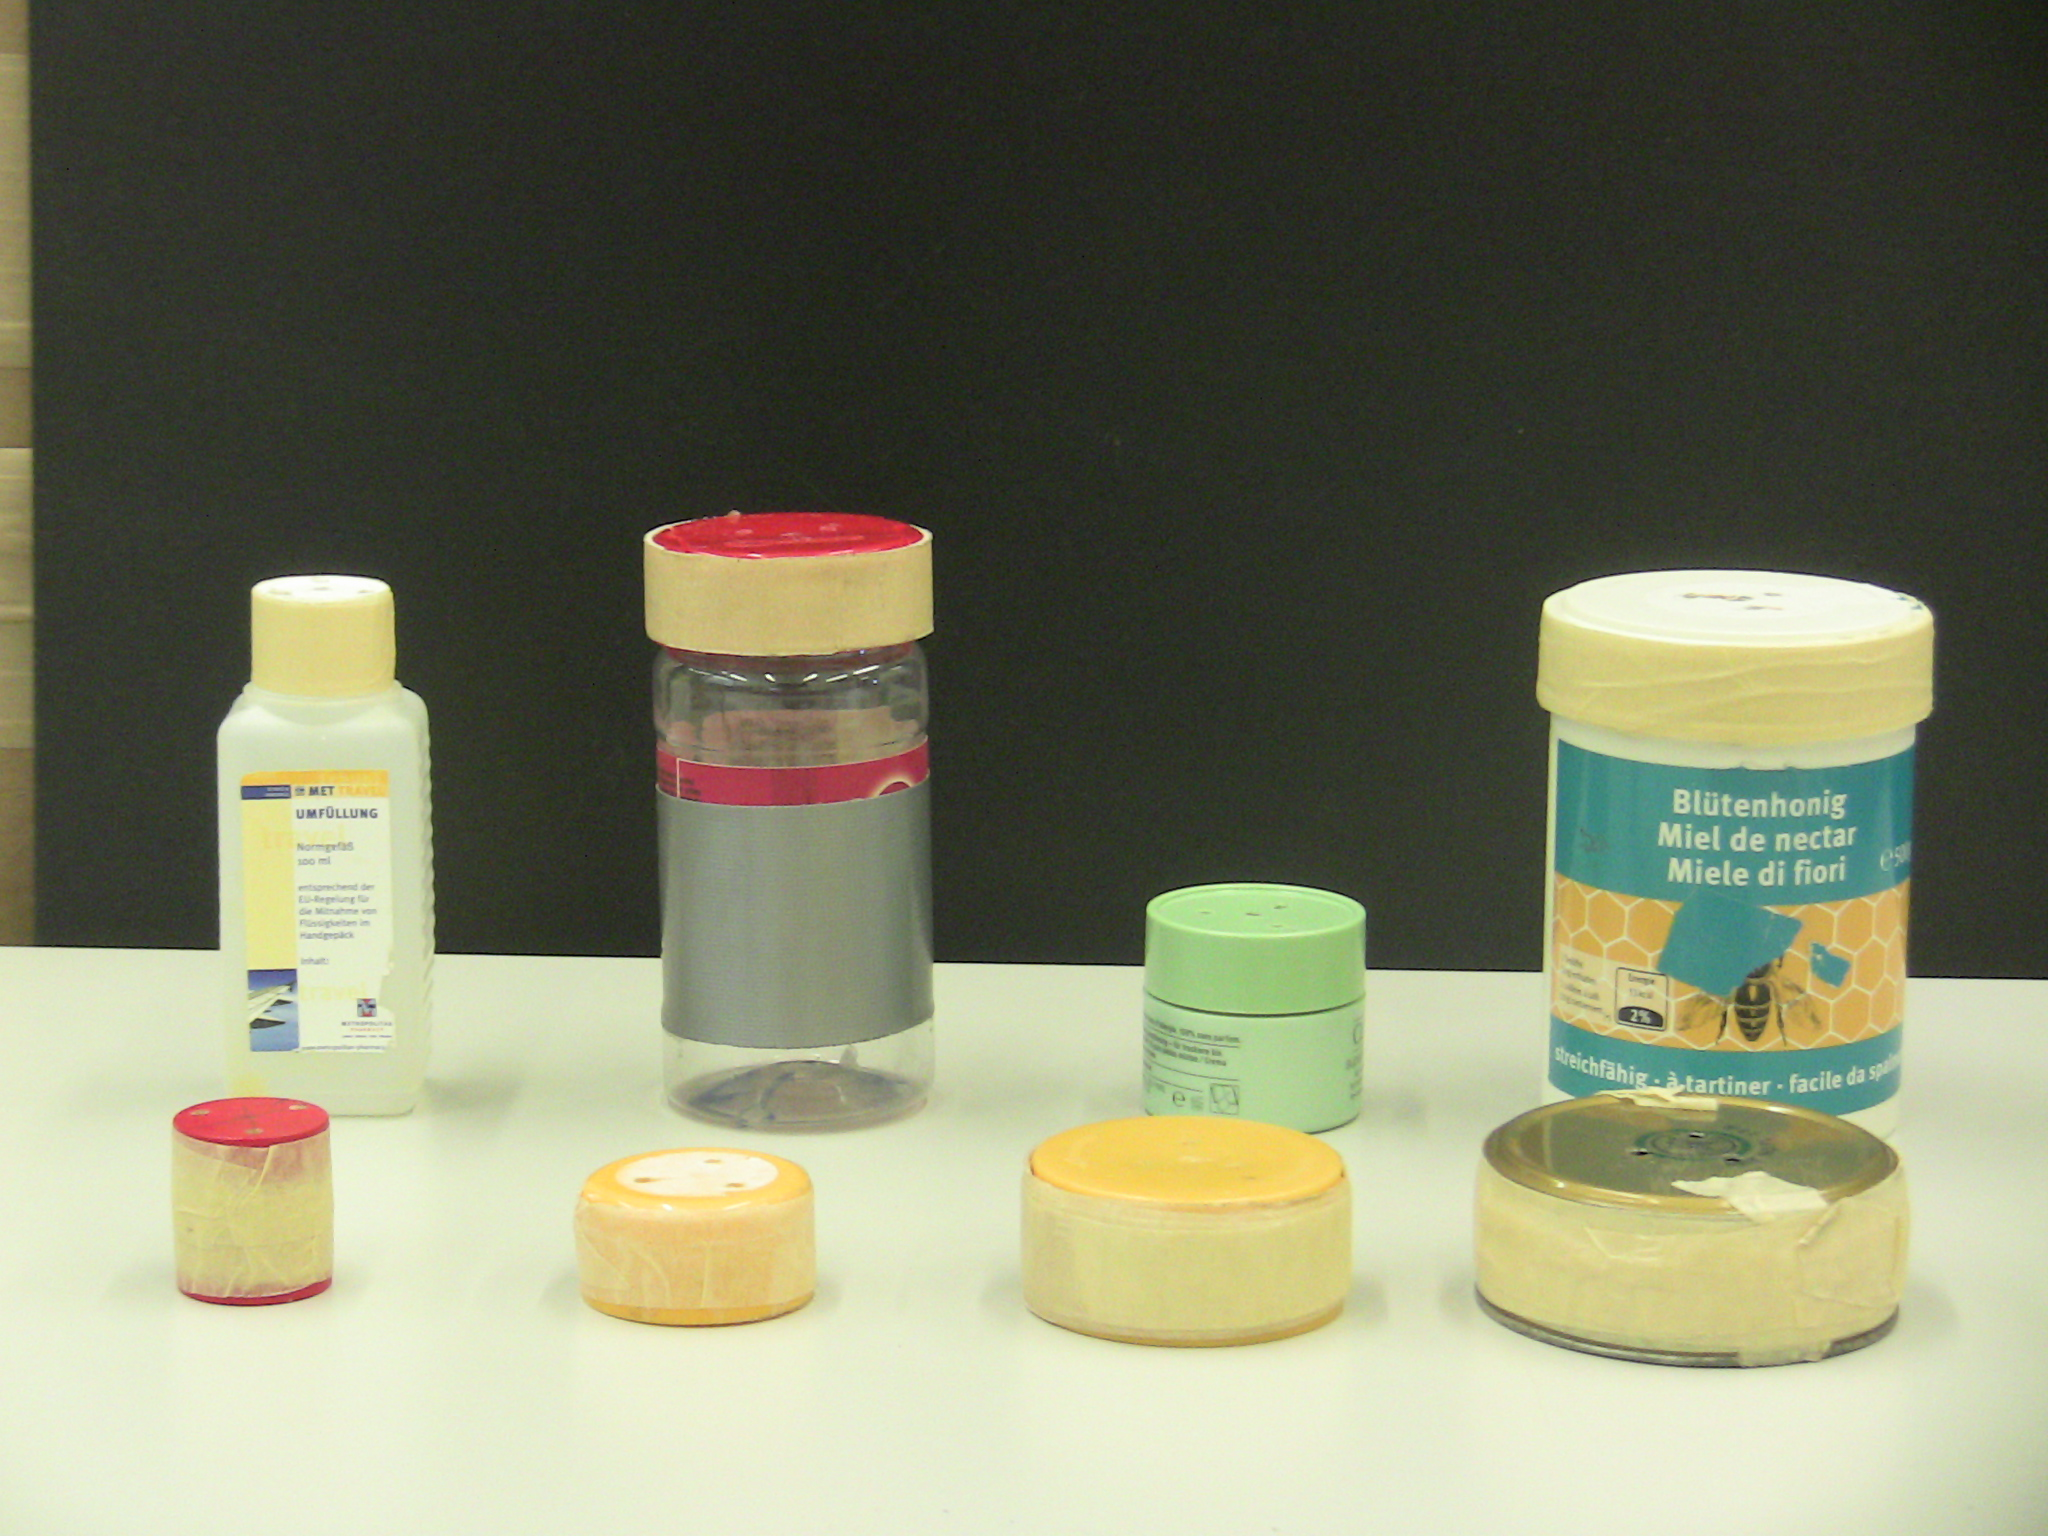
\includegraphics[width=10cm]{./fig_cha4/b_c.jpg}
  \caption{ \scriptsize{Bottles and caps for human demonstration. From left to right: b1 c1, b2 c2, b3 c3, b4  c4}
}
\label{fig:b_c}
\end{figure}






% 25,42,56,80,110, c1-c5, mm
\begin{table}
\center
\caption{Different setups of bottles and caps for demonstration. Bottle 1 to 4 are in increasing order of the difficulty to open. Cap 1 to 4 is in increasing order of the cap sizes, whose diameters are shown.}
\begin{tabular}{p{2cm}|p{1.5cm} |p{1.5cm} |p{1.5cm} |p{1.5cm}}

%\backslashbox{}{}
                                & \parbox[c]{1em}{ 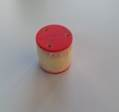
\includegraphics[width=1.5cm]{./fig_cha4/c1.jpg}}
                                & \parbox[c]{1em}{ 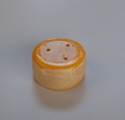
\includegraphics[width=1.5cm]{./fig_cha4/c2.jpg}}
                                & \parbox[c]{1em}{ 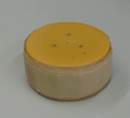
\includegraphics[width=1.5cm]{./fig_cha4/c3.jpg}}
                                & \parbox[c]{1em}{ 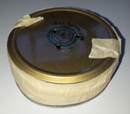
\includegraphics[width=1.5cm]{./fig_cha4/c4.jpg}}  \\
    & Cap 1  25$mm$ & Cap 2  42$mm$ & Cap 3  56$mm$ & Cap 4  80$mm$ \\
\hline
\parbox[c]{1em}{ 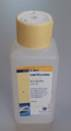
\includegraphics[width=1.5cm]{./fig_cha4/b1.jpg}} & & &b1c3 &\\
Bottle 1 & & & &\\
\hline
\parbox[c]{1em}{ 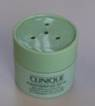
\includegraphics[width=1.5cm]{./fig_cha4/b2.jpg}} & & & &\\
%Bottle 2 & b3c1& b3c2& b3c3& b3c4\\
Bottle 2 & & & b2c3&\\
\hline
\parbox[c]{1em}{ 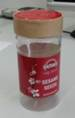
\includegraphics[width=1.5cm]{./fig_cha4/b3.jpg}} & & & &\\
%Bottle 3 & & & b3c3&\\
Bottle 3 & b3c1& b3c2& b3c3& b3c4\\
\hline
\parbox[c]{1em}{ 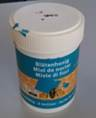
\includegraphics[width=1.5cm]{./fig_cha4/b4.jpg}} & & & &\\
Bottle 4 & & & b4c3&\\
\hline
\end{tabular}
\label{bottlesandcaps}
\end{table}

\begin{figure}
  \centering
  \subfloat[\scriptsize{}]  {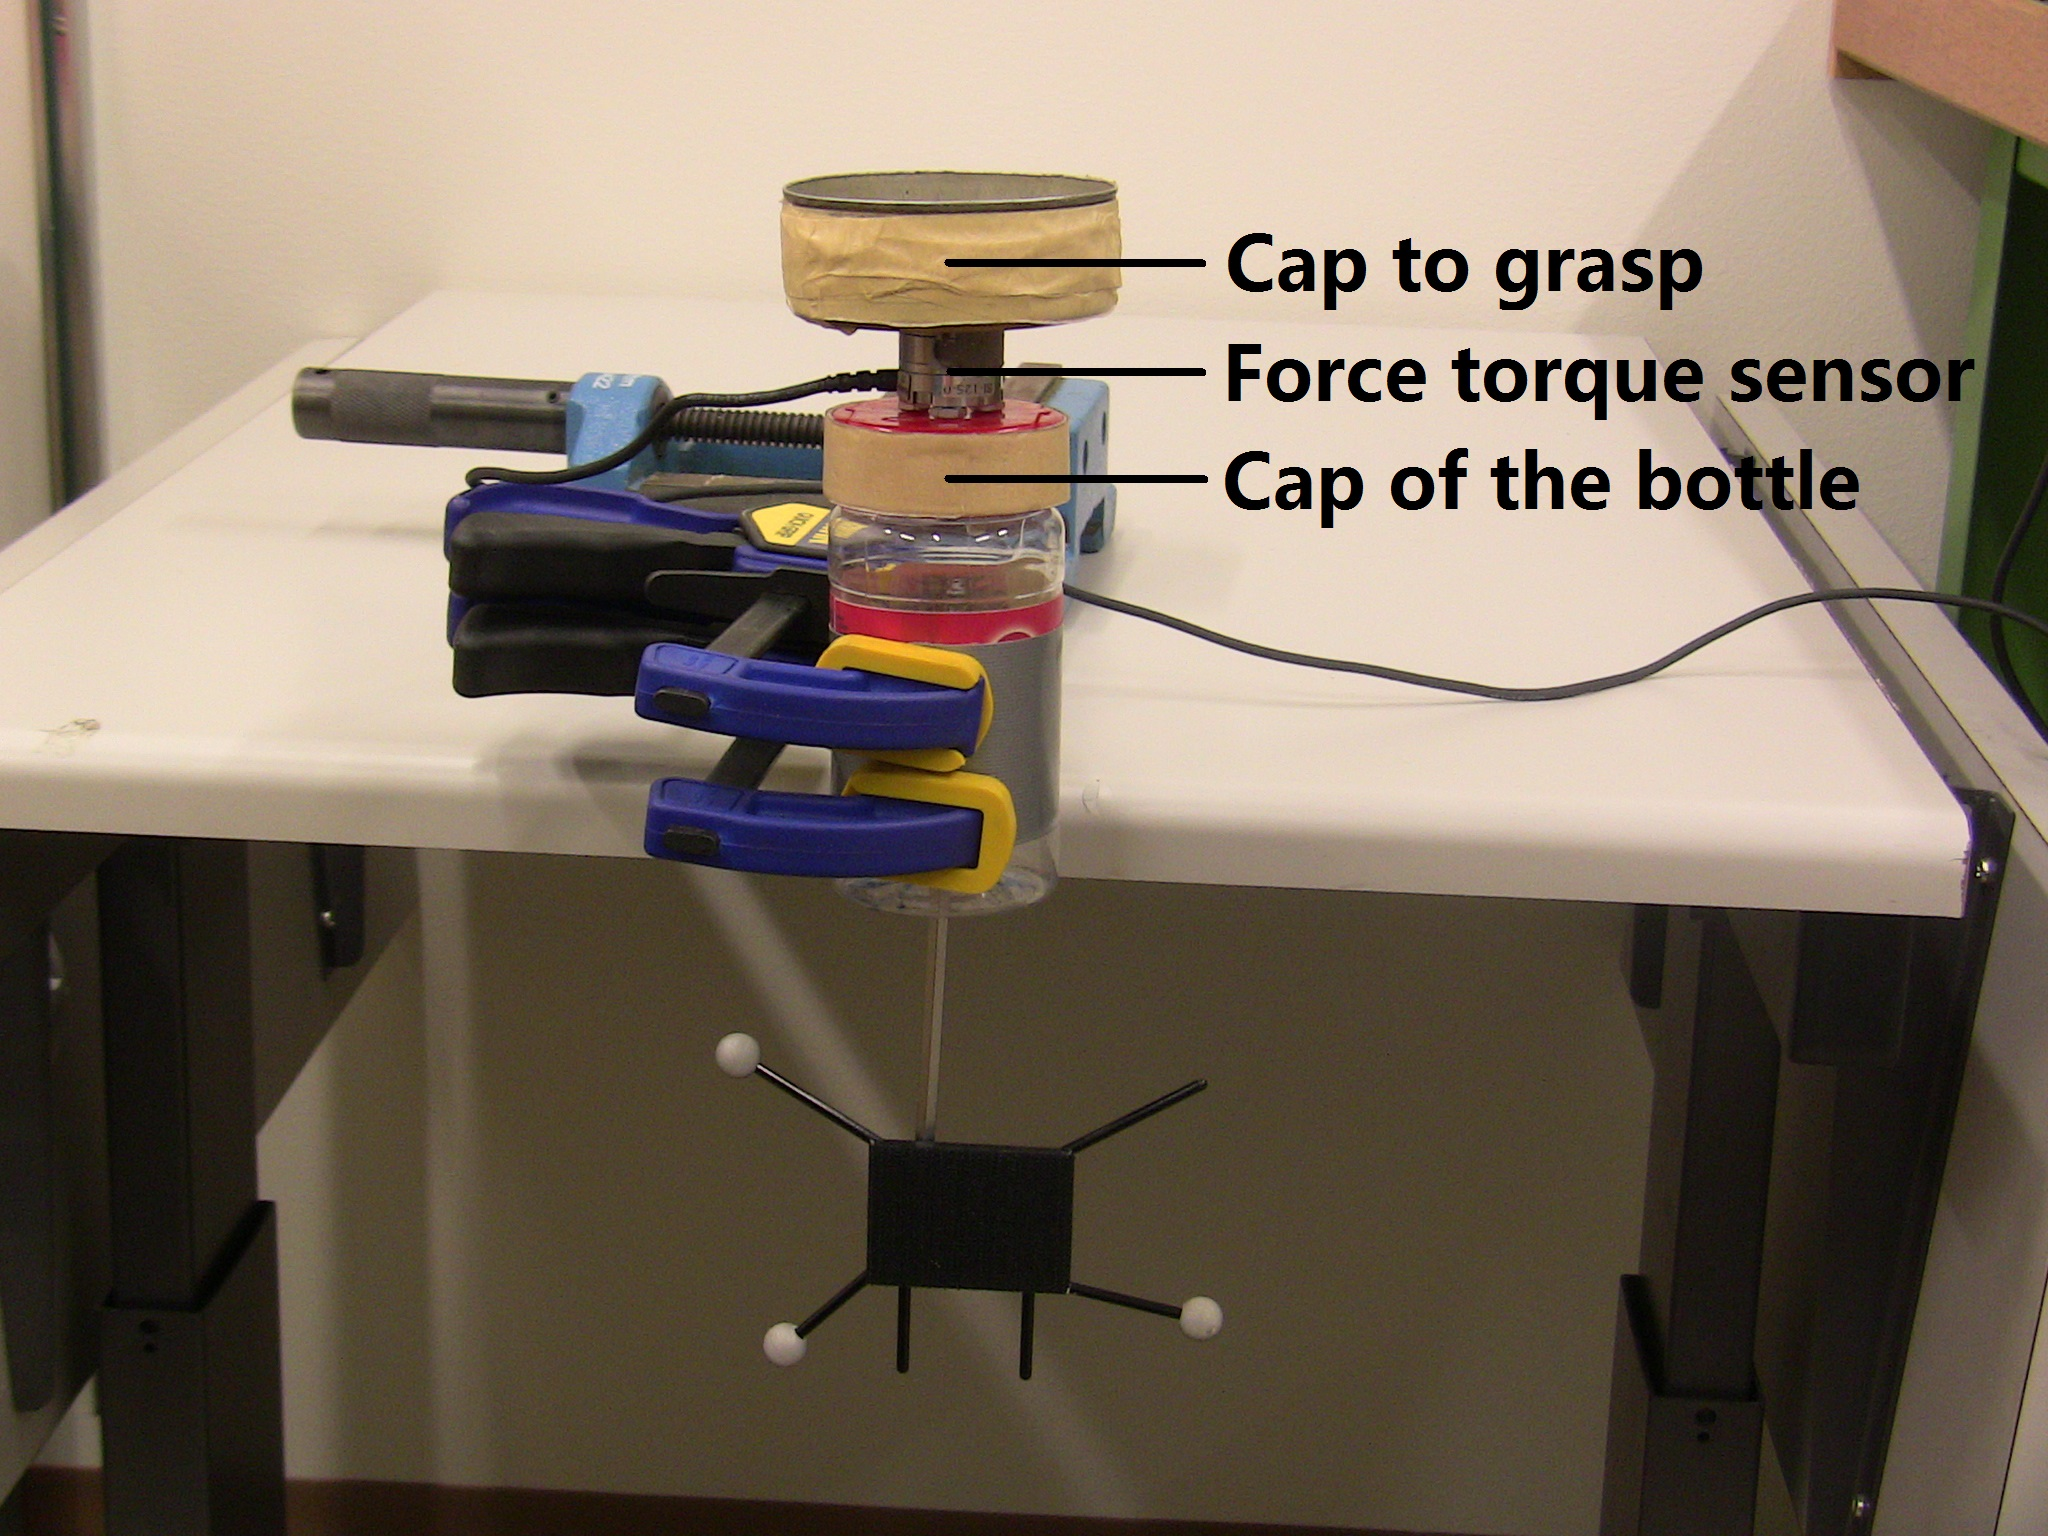
\includegraphics[width=6cm]{./fig_cha4/setup2_3.jpg}}
  \hspace{1cm}
  \subfloat[\scriptsize{}]  {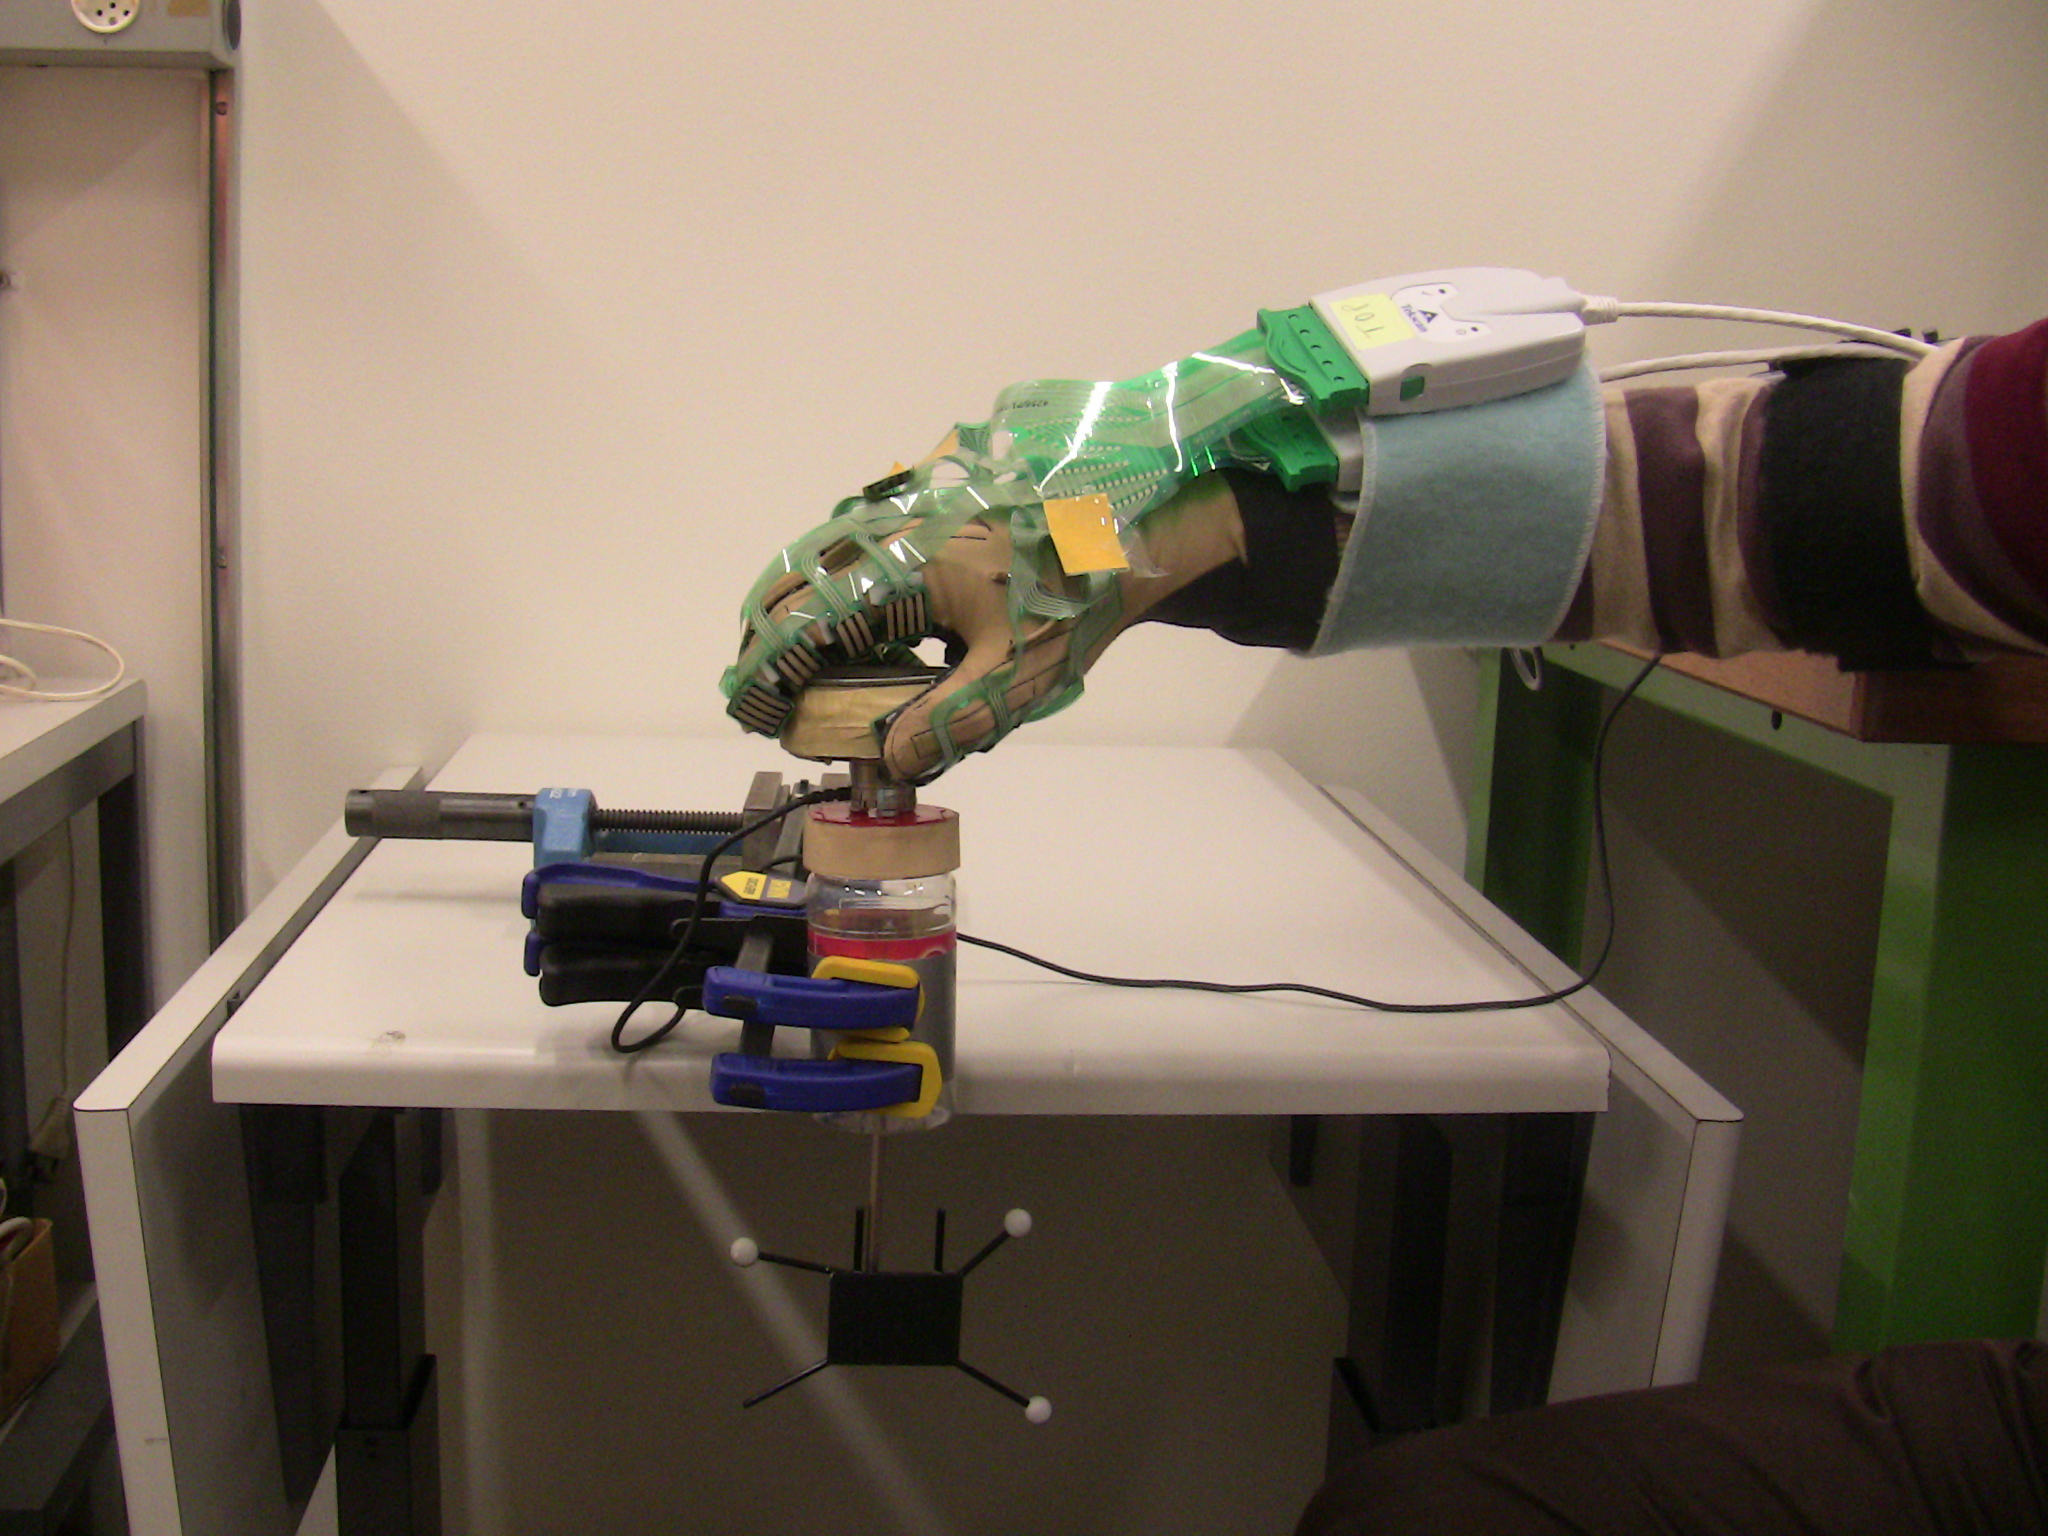
\includegraphics[width=6cm]{./fig_cha4/demo.jpg}}
  \caption{ \scriptsize{Experimental setup for the task of opening a bottle cap. (a) Setup b3c4: bottle 3 combined with cap 4 (cap to grab). A force-torque sensor is mounted between the ``cap of the bottle'' and the ``cap to grab'', so that the exert force and torque can be measured. A set of Optitrack markers are connected with the cap to record the displacement of it. The bottle is fixed on a table. (b) Human demonstrating opening a bottle cap. To avoid extra torque, only one hand is used during the demonstration. Human grip the cap from the top and apply torque to the system. }
}
\label{fig:setup}
\end{figure}

\subsubsection{Sensors}
\label{cha4:sec3:experimentsetup:sensor}
In each setup the demonstrator demonstrates the task of opening bottle
cap three times. Before each demonstration, the bottle is tighten with
the cap with the same scale of tightness. In total we recorded 21~sets
of demonstrations. In this section, we the sensor recording of these
demonstrations.



As explained in section~\ref{cha4:sec2:learn:objectlevel}, we focus on the tuple $\{\tau,F,s\}$ of the task. Three different set of sensors are used in the experiment to capture them:

\begin{enumerate}
\item Force torque sensor\footnote{https://www.ati-ia.com/} for exerted torque ($\tau$);
\item OptiTrack\footnote{http://www.naturalpoint.com/optitrack/} for cap displacement ($s$);
\item Tekscan\footnote{http://www.tekscan.com/} for exerted force ($F$).
\end{enumerate}

Data from these three sensors stream from three different
channels. Due to hardware limitations, the raw data steam from the
different channels does not come at the same time, and cannot be
recorded at a regular frequency. To synchronize the data, we produce a
synchronization signal at the beginning of each demonstration: the
demonstrator taps on the cap three times. The movement of the hand and
impulses on the cap produce simultaneous pulses in all three
channels. After recording, the data from the different channels is
synchronized by aligning the synchronization signal.

In this task, the turning torque is the essential variable. This is
measured and recorded by an ATI force torque sensor. It is mounted
between the bottle and the cap (Figure.~\ref{fig:setup}). During the
task, the demonstrator grasps the cap on the top of the force-torque
sensor and applies torque to open the bottle mounted below the
sensor. As the bottle is fixed to the table, the movement of the cap
is restricted to the rotation along the bottle's axis. Under the
approximation of zero angular momentum, the reading of the sensor
shows the force and torque applied to the cap. Besides the torque,
force applied to the z-axis direction is also recorded for the purpose
of synchronization  (Section~\ref{cha4:sec3:dataanalysis}).

We track the displacement of the cap by a motion tracking system OptiTrack. The OptiTrack system tracks movement by the infra-red reflecting markers attached to the object. In order to avoid obstacle during the demonstration, we attach markers to a stick, which is fixed to the cap from one end and the other end coming out from the bottom of the bottle (Fig.~\ref{fig:setup}). We also recorded the human hand movement, by tracking the markers attached to the human hand. The movement of human hand is used later for synchronization (Section~\ref{cha4:sec3:dataanalysis}).

During the task, the human also applies grip force on the cap in order
to grasp it firmly for turning. This force cannot be sensed by the
force torque sensor. Therefore, we used a pressure sensor (Tekscan
Grip System) for measuring the grip force. The Tekscan Grip System is
a flexible tactile pressure sensor that can be built into a glove. It
has 18~patches of sensors to cover the human's hand's front
surface. For manipulation, humans use not only the front surface, but
also the side surface of our fingers. In order to measure the force
applied by those surfaces, we mount two sets of Tekscan Grip System
sensors onto a glove to cover also the side surfaces
(Figure.~\ref{ftsensor}). The method of mounting the sensors to the glove
is detailed in~\citep{deSouza2014}. With different sizes of the caps
or in different stages of the task, the way a human grasps the cap may
vary.  For example, a human may use two fingers to grip the smallest
cap~$c1$, and four fingers to grip the biggest cap~$c4$. The patches
receiving contact in each grasp are recorded. In the computation of
the total grip force, only the patches used are taken into
account. All patches are calibrated to give readings in the unit of
$N{\cdot}m$.


\subsection{Data Analysis}
\label{cha4:sec3:dataanalysis}
% Data: how to compute the cap displacement. Hand position. compute contact force.
In this section we explain how we manage the raw data and extra
training data.  The raw data from the three sensors streams is in
three separate channels. Each stream has a different format and hence
is handled differently.


\paragraph{\textbf{Exerted torque}}
\label{ftsensor}
As the movement of the cap is restricted to rotation around the
z-axis, we are concerned only with the torque applied in this direction.
Another dimension of concern is the force applied in the z direction. The
three taps on the cap before each demonstration will create three
pulses in the z direction and hence is used for synchronization.


\paragraph{\textbf{Object displacement}}
\label{sec:optiktrack}
From the OptiTrack, the cap's displacement is originally expressed in
the position vector and the rotation matrix. The angular
displacement of the cap is computed by the rotation matrix of the cap, and
the hand movement by the position vector of the hand. The accumulated
angular displacement is used to learn the model and the hand movement
is used to synchronize the data.



\paragraph{Tekscan}

As mentioned in previous section, we used two sets of Tekscan to cover
the front and the side of the human hand. This enables the
demonstrator to use any grasp they like for the task --- the human was
not restricted to using just two or three fingers as is the case in
most other grasping experiments. For each type of grasp, the reading
from the patches contacting with the cap are summed and multiplied by
their surface area to compute the total grip force.

Data from these three channels is synchronized by aligning the
synchronization pulses. The time of the last detected pulse is set as
the zero-reference point. After synchronization we re-sample all the
temporal sequences to 100Hz. Thus each single data point is
synchronized. Finally, we filter the noise by a low pass
filter. Figure~\ref{fig:3channels} shows an example of the data from
three different channels.




\begin{figure}
  \centering
  \hspace{-1cm}
  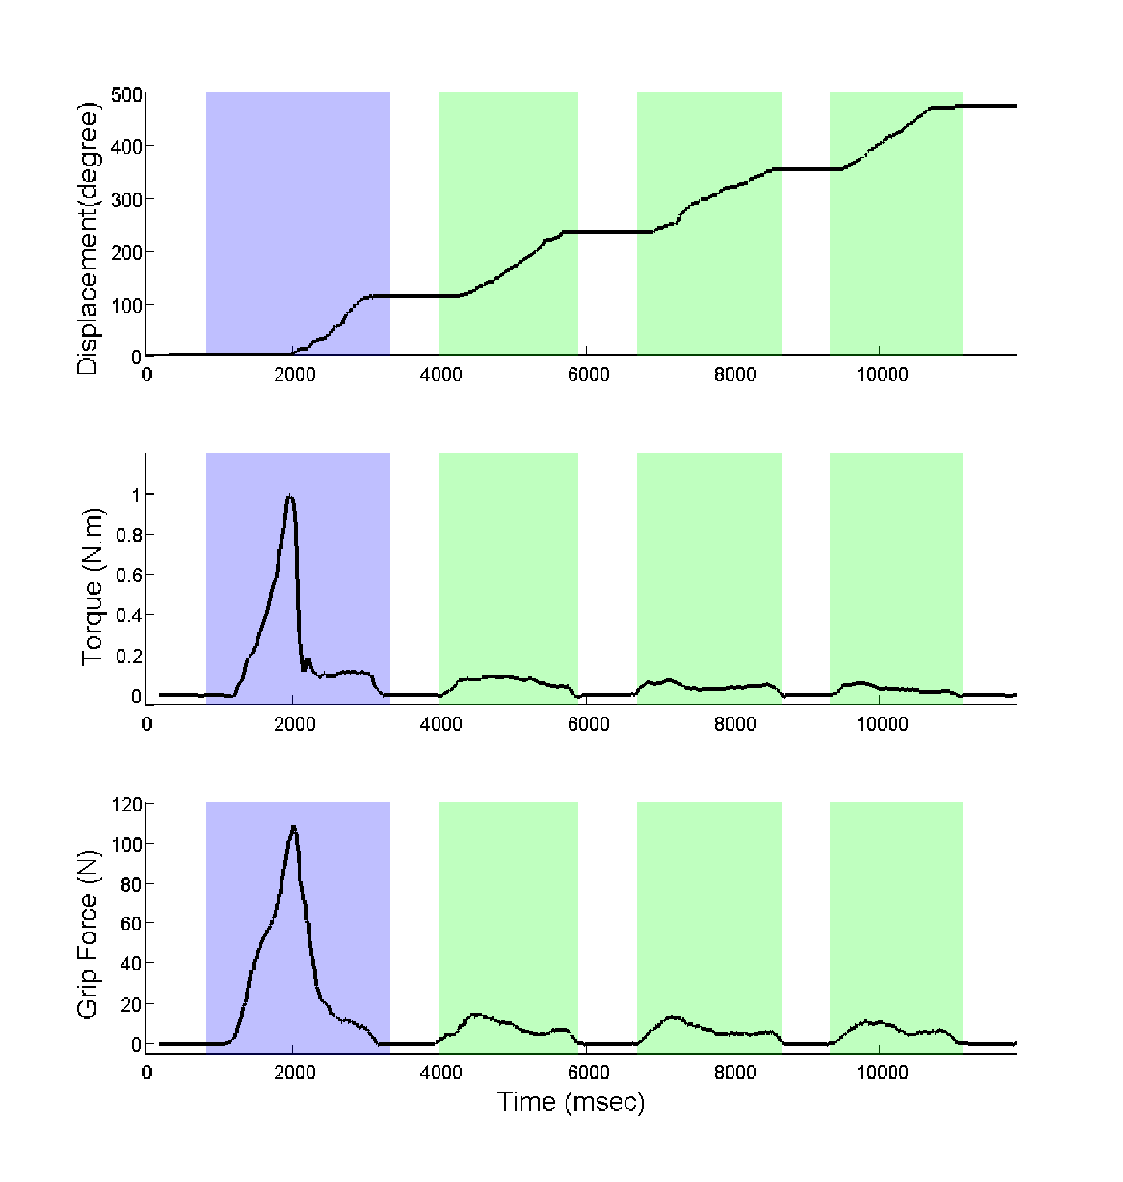
\includegraphics[width=14cm]{./fig_cha4/b3c2_1_sTF.pdf}
  \vspace{-0.5cm}
  \caption{ \scriptsize{Aligned data of all three channels. Highlighted parts mark the turning process: blue blocks denote the first cycle, i.e. the phase I, and green blocks denote the later cycles, i.e the phase II. Phase I is significantly different from the phase II.}
}
\label{fig:3channels}
\end{figure}

% Only turning cycle
In this task we focus on the turning stage of each cycle. More specifically, we focus on the data starting from the moment that the fingers contact the cap and end at the moment that the turning is finished and the cap is released. The reaching and releasing cycles do not involve contact with the environment and hence are not of concern here.
% segmentation is not our job
In order to collect data from only the turning cycles, we trim the data by the contact signal: only parts of the sequence with non-zero contact force will be kept.\footnote{In this task the segmentation is done manually. The data can also be segmented by other algorithms but here we do not focus on task segmentation.} The trimmed sequences are labeled by their associated equipment setup and the order in which they occur, e.g. the first cycle of the bottle~1 with cap~3 is labeled by $b1c3\_1$.

As can be seem from Fig.~\ref{fig:3channels}, there are dramatic difference between the cycle one and the rest of the cycles: the exert force and torque are much higher in the first cycle than in the other cycles. This is caused by the difference between the static friction and the kinetic friction. At the beginning of the task we have to first break the contact between the bottle and the cap. The friction we need to break at this stage is decided by the static FCO. Once the cap starts to move, the FCO between bottle and cap transits to kinetic FCO, which is usually smaller than the static FCO for the same surface condition. As a result, the torque and hence the grip force required to turn the cap decrease in the later cycles. This phenomenon implies that at lease two modules are needed for this task. In the later section we will discuss these two phases separately and refer the cycle one as ``phase I'' and the later cycles as ``phase II''.

In different demonstrations, the number of cycles used to open the cap is different, varying from four to six. The pattern of the later cycles are similar as the demonstrator just repeats the same strategy for rotating the cap. For training, we take the first four cycles from each of the demonstrations. As mentioned above, human demonstrate the task in seven different setups, each for three times. This results in 84~time series in total for the learning.

%% what was recorded
%In each demonstration, data from first time the hand grab the cap to the cap is finally open and lifted, was record. Opening bottle cap is a cyclic task, each cycle of which includes reaching, turning and releasing stages. Depending on the tightness of the cap, a few cycles need to be done before the bottle is open. In this task we focus on the turning stage of each cycle, which start from the time that the fingers contact the cap and end at the moment that the turning is finished and the cap is released. During the turning cycles, force and torque are applied to the cap in order to break it's contact with the the bottle and the dynamics of the system changes diametrically. Our goal is to learn a model to encode human's strategy to cope with the abruptly changing environment during the turning cycle. The reaching and releasing cycles do not involve contact with the environment and hence we omit them.







\subsection{Learning Modules}
\label{cha4:sec3:learning}

In this section, we explain how we encode the training data into a few different modules. As mentioned in Section~\ref{cha4:sec2:learn}, the first step is to cluster the data and find out the number of modules required in this task (Section~\ref{cha4:sec3:learning:clustering}). After that, a forward model and an inverse model is built for each module (Section~\ref{cha4:sec3:learning:module}) and we use these modules to generate motor commands.

\subsubsection{Data clustering}
\label{cha4:sec3:learning:clustering}
To cluster the 84 time series $Q\{s,\tau,F\}$ obtained from human demonstration, we first compute the distance between each pair of them by the DTW technique. As this task is time independent, ``warping'' of the data in the dimension of time does not effect the control policy encoded in the time series. The distances between each pair of the time series is shown in the heatmap (Fig.~\ref{fig:heatmap}). As can be seen from the heatmap, the trials with the same setup and in the same cycle are very similar to each other. Hence we regard these trials a representing the same control strategy and use their variance as the criterion of the clustering. From this heatmap we can also see that within the same cycle, the trials with the same bottle but with different caps, e.g. $b3c1, b3c3$ and $b3c4$, are similar to each other. In the first cycle, the trials with the same cap but with different bottles, e.g. $b1c3, b2c3, b3c3$ and $b4c3$, are significantly different from each other. In the the later cycles, this differences decrease gradually. This result shows that in the opening bottle cap task, the surface condition between the bottle and the cap plays an important role in the control strategy, while the role of cap size is relatively minor. Figure~\ref{fig:cappatterns} shows three trials of opening bottle b2 with different sizes of caps. It can be seen that their patterns are similar.

\begin{figure*}
\label{heatmap}
  \centering
  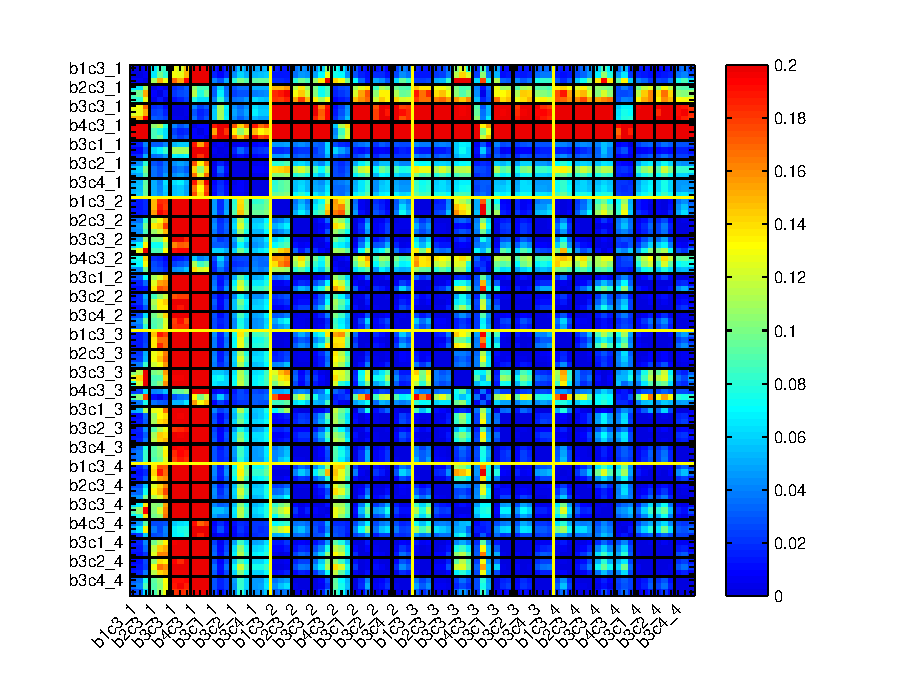
\includegraphics[width=18cm,height=18cm]{./fig_cha4/heatmap_all6_3.eps}
  \caption{ \scriptsize{A heatmap representation of the distance matrix of 84 time series (7 setups $\times$ 4 cycles $\times$ 3 trials). The labels are in the format of ``setup$\_$cycle''. For example, ``b1c2$\_$1'' represents the first cycle of the b1c2 setup. The yellow lines divide the x and y axis by the 4 cycles and hence form 16 big blocks. In each big block, the black lines divide the x and y axis by the 7 setups and hence form 49 small blocks. }
}
\label{fig:heatmap}
\end{figure*}

\begin{figure}
    \centering
    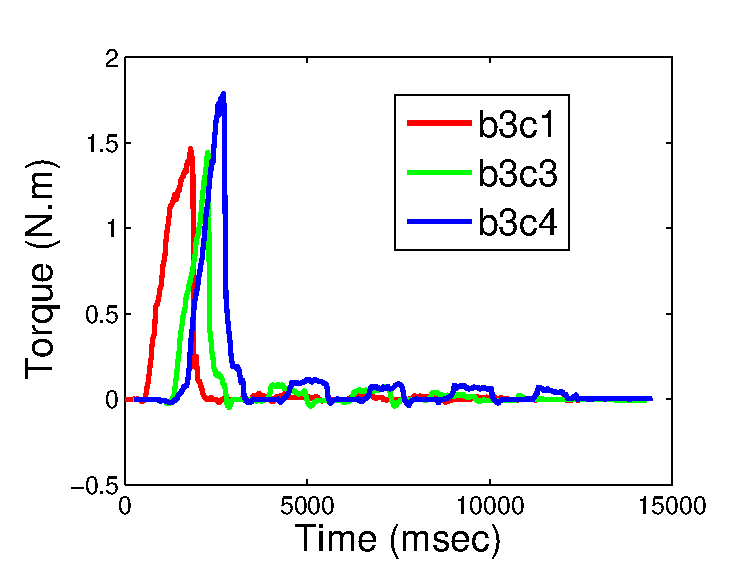
\includegraphics[width=12cm]{./fig_cha4/c1c3c4_time_T.eps}
    \caption{ \scriptsize{Exert torque for opening bottle b3 with three different cap sizes.}
}
\label{fig:cappatterns}
\end{figure}


As mentioned before, the demonstration of each setup is repeated three times and the data from the same setup and same cycle are presumed to belong to the same cluster. To set a threshold for clustering, we check the distances between the time series come from the same setup and the same phase. The largest distance found is 0.04 (normalized) from the $b3c2$ phase 4. We add a $10\%$ margin on this (resulting in 0.044) and use it as the threshold of clustering. The time series distances less than the threshold are grouped into the same cluster. We use the hierarchical agglomerative clustering (Section~\ref{cha4:sec2:learn:cluster}) to merge the data into different clusters. After 5 times of merging, the clusters are not merge-able and 3 clusters remain.

These three clusters contain the data from:

\begin{enumerate}
\item phase I of $b4c3$ (most difficult bottle), 3 time series;
\item phase I of $b3c1, b3c2, b3c3, b3c4, b2c3$ and phase II of $b4c3$, 24 time series;
\item phase I of $b1c3$ (easiest bottle) and phase II of the other setups, 57 time series.
\end{enumerate}

The result of clustering is shown in Table~\ref{tab:cluster}. This result suggests that humans use three different strategies for opening bottles: one for handling the phase I of the most difficult bottle with adhesive materials on the bottle and cap surfaces; one for handling the phase I of most bottles and the phase II of the most difficult bottle; and one for handling the phase I of the lubricated bottle and the phase II of the other bottles. The size of the cap turns out to be playing a less important role in the control strategies. According to this result, we encode these three clusters separately.



\begin{table*}
\caption{Clustering results}
\begin{tabular}{p{1.6cm} p{1.6cm}|p{2cm} p{2cm} p{2cm}  p{2cm} }
& & \parbox[c]{1em}{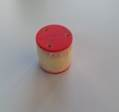
\includegraphics[width=1.5cm]{./fig_cha4/c1.jpg}}\newline Cap 1
& \parbox[c]{1em}{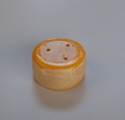
\includegraphics[width=1.5cm]{./fig_cha4/c2.jpg}}\newline Cap 2
& \parbox[c]{1em}{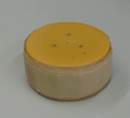
\includegraphics[width=1.5cm]{./fig_cha4/c3.jpg}}\newline Cap 3
& \parbox[c]{1em}{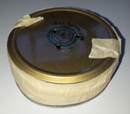
\includegraphics[width=1.5cm]{./fig_cha4/c4.jpg}}\newline Cap 4      \\ \hline
{\parbox[c]{1em}{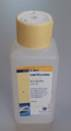
\includegraphics[width=1.5cm]{./fig_cha4/b1.jpg}}}
         & Phase I  &           &           & {\vspace{-0.7cm}}\pbox{2cm}{(b1c3) \\ Cluster 3} &           \\
Bottle 1 & Phase II &           &           &        Cluster 3 &           \\ \hline

{\parbox[c]{1em}{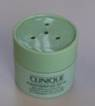
\includegraphics[width=1.5cm]{./fig_cha4/b2.jpg}}}
%         & Phase I  &{\vspace{-0.7cm}}\pbox{2cm}{(b3c1) \\Cluster 2} &{\vspace{-0.7cm}}\pbox{2cm}{(b3c2) \\Cluster 2} &{\vspace{-0.7cm}}\pbox{2cm}{(b3c3) \\Cluster 2} &{\vspace{-0.7cm}}\pbox{2cm}{(b3c4) \\Cluster 2} \\
%Bottle 2 & Phase II &       Cluster 3 &       Cluster 3 &       Cluster 3 &       Cluster 3 \\ \hline
         & Phase I  &           &           &{\vspace{-0.7cm}}\pbox{2cm}{(b2c3) \\Cluster 2} &           \\
Bottle 2 & Phase II &           &           &       Cluster 3 &           \\ \hline

{\parbox[c]{1em}{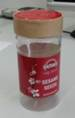
\includegraphics[width=1.5cm]{./fig_cha4/b3.jpg}} }
%         & Phase I  &           &           &{\vspace{-0.7cm}}\pbox{2cm}{(b3c3) \\Cluster 2} &           \\
%Bottle 3 & Phase II &           &           &       Cluster 3 &           \\ \hline
         & Phase I  &{\vspace{-0.7cm}}\pbox{2cm}{(b3c1) \\Cluster 2} &{\vspace{-0.7cm}}\pbox{2cm}{(b3c2) \\Cluster 2} &{\vspace{-0.7cm}}\pbox{2cm}{(b3c3) \\Cluster 2} &{\vspace{-0.7cm}}\pbox{2cm}{(b3c4) \\Cluster 2} \\
Bottle 2 & Phase II &       Cluster 3 &       Cluster 3 &       Cluster 3 &       Cluster 3 \\ \hline

{\parbox[c]{1em}{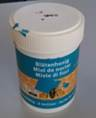
\includegraphics[width=1.5cm]{./fig_cha4/b4.jpg}}\newline }
         & Phase I  &           &           &{\vspace{-0.7cm}}\pbox{2cm}{(b4c3) \\Cluster 1} &           \\
Bootle 4 & Phase II &           &           &       Cluster 2 &           \\ \hline
\end{tabular}
\label{tab:cluster}
\end{table*}



\subsubsection{Learning Modules}
\label{cha4:sec3:learning:module}
We encode the data in each of the modules using GMM. As explained in Section~\ref{cha4:sec2:learn}, a forward model and an inverse model are built for each module. The forward model is encoded by the joint distribution $p\{s(t),s(t-1),a(t-1)\mid\Omega_F\}$, while the inverse model is encoded by $p\{s(t),s(t+1),a(t),a(t-1)\mid\Omega_I\}$. For each model, the number of Gaussians is determined by the BIC. We use 25 Gaussians for cluster 1, 40 for cluster 2 and 15 for cluster 3. Their BIC tests are shown in Fig~\ref{fig:bic}.

\begin{figure}
  \centering
  \includegraphics[width=6cm]{./fig_cha4/bic_cluster1.eps}
  \includegraphics[width=6cm]{./fig_cha4/bic_cluster2.eps}
  \includegraphics[width=6cm]{./fig_cha4/bic_cluster3.eps}
  \caption{ \scriptsize{BIC test result for clusters. (a) Cluster 1, (b) Cluster 2, (c) Cluster 3.}
}

\label{fig:bic}
\end{figure}

%\begin{table}
%\centering
%\renewcommand{\arraystretch}{1.5}
%    \begin{tabular}
%    %{|>{\centering\arraybackslash}p{2cm}|>{\centering\arraybackslash}p{1.2cm}|>{\centering\arraybackslash}p{1.7cm}|>{\centering\arraybackslash}p{1.2cm}|>{\centering\arraybackslash}p{1.5cm}|>{\centering\arraybackslash}p{1.5cm}|>{\centering\arraybackslash}p{1.7cm}|>{\centering\arraybackslash}p{1.7cm}|>{\centering\arraybackslash}p{0.9cm}|}
%    { | c | c | c | c | c |}
%    \hline
%    Cluster & Forward Model &  Inverse Model \\ \hline
%    1       & 98.1\%  & 13.8     \\ \hline
%    2             & 92.1\%  & 21.9    \\ \hline
%    3              & 91.0\%  & 16.0    \\ \hline
%    \end{tabular}
%\caption{Number of Gaussians in each GMM}
%\label{tab:GMM}
%\end{table}


\subsection{Generating motor commands for manipulation}
\label{cha4:sec3:command}
%\label{sec:command}
Our approach is independent of the robot system and can potentially be applied to any robot. We chose to implement this work with a Barrett hand mounted on a KUKA lightweight robot as they are available in our lab. We implemented the multiple module system on this platform to enable the robot to open bottle caps.

\begin{algorithm}
  \caption{Control Algorithm}
  \begin{algorithmic}[1]
    \For{r = 1:4}
    \State REACHING(): Robot moves to initial position\;
        \Function{TURNING()}{} %      \Comment{$\oplus$: bit}
          \State Read previous sensor information $\{s_{t-1},\tau_{t-1},F_{t-1}\}$\;
          \For{k=1:3}
            \State $\hat{s}^{k}$ = FORWARD($s_{t-1},T_{t-1},\Omega_I^k$) \;
          \EndFor
          \For{k=1:3}
            \State $\lambda{k}$ = ResponsibilityFactor($\hat{s}^{k},s_t$) \;
          \EndFor
          \State Read current sensor information $\{s_{t}\}$\;
          \For{k=1:3}
            \State $\{a^k\}$ = INVERSE($s*_{t+1},s_t,a_{t-1}$) \;
          \EndFor
          \State $\{a_t\} = \sum_{k=1,2,3}\lambda{k}\{a^k\}$\;\;
          \State Add compensational torque to $\tau_t$\;
          \State Execute motor command $\{a_t\}$ \;
          \State RELEASING(): Release the cap;
        \EndFunction
    \EndFor

    \While{LIFTCAP() is false}
        \State REACHING();
        \State TURNING();
        \State RELEASING();
    \EndWhile

  \end{algorithmic}
  \label{code:control}
\end{algorithm}


In this experiment, we control the wrist joint (last joint of KUKA) for producing torque to turn the bottle cap. A force torque sensor is fixed under the bottle to provide torque feedback. Each finger of the Barrett hand is mounted with a $Syntouch$\footnote{http://www.syntouchllc.com/} tactile sensor, which is calibrated to provide contact force information, for the grip force feedback. The cap displacement is measured by the wrist joint displacement, assuming that there is no slip between the fingers and the cap.

The target bottle is fixed on the top of a table with it's cap tightened. The robot is placed above it at a distance that allows a proper grasp on the cap. The Barrett hand then close the fingers until the bottle cap is touched. This position is recorded as the initial position, where the cap displacement is marked as zero. In the experiment we focus on the turning cycle. The releasing and reaching cycles are programmed by opening the fingers and restoring to the initial position.

We first test the model with the trained bottles and then test with two new bottles. With each bottle, the turning-releasing-restoring cycles are repeated four times. Data streams from the sensors are filtered to $100Hz$. Once the turning cycle starts, the forward models take the torque and displacement at the last time step as input, and compute the expected displacement of the current time step. These expected displacements are compared with the actual displacement measured at the sensor to evaluate the reliability, expressed as a normalized responsibility factor, of each module. The inverse models take the current displacement, desired next displacement and the previous force and torque as input to compute the proper action (force and torque) to take on the cap. Each of the three outputs is multiplied with its responsibility factor, and the final output is the sum of the factorized three outputs (Algorithm~\ref{code:control}).

In implementation on a real robot, we found that without putting any restriction of the responsibility factor, it can change rapidly. This is caused by the environmental noise in the sensory input and results in instability of the control system. We apply a low pass filter on the responsibility factor to reduce the fluctuation. This filtering implies that the real dynamics does not switch with high frequency, which is consistent with the character of our task.


Before applying the final output on the robot, a compensational torque is added to it in order to compensate the lag causing by the distortion of the robot hand during turning. The control algorithm described above is shown in algorithm~\ref{code:control}.



\subsection{Experiment results}
\label{cha4:sec3:result}

% TODO:
% 1) explain whether the use of the clusters correspond to your expectations and really relate to an identification of different phases
% 2) what the novel object consist of, in what do they differ from the other objects
% 3) what were your expectations in terms of cluster use for these new objects
% 4) Do the results match your expectations

%We implement this algorithm with two bottles (b1 and b4) in the training set and then two bottles (b5 and b6) had not been used for training.
We validated the algorithm to control cap opening in our robot. We first tested the ability of the system to open 2 of the bottles seen during training (b1 and b4). We then tested the generalization capacity of the system by opening two bottles (b5 and b6) not seen during training.
Bottle b1 and b4 are the easiest and most difficult bottles to open in the training set.
Bottle b5 is a large bottle, which is hard for a human to grab and open. Bottle b6 is a glass bottle with a plastic cap. The surface interaction between these two materials is not demonstrated. As the Barrett hand is significantly larger than a human hand, $b1, b4, b6$ are mounted with $c5$ (the cap of $b5$ with diameter $110 mm$) on the top to ensure a firm grasp. In total 4 different setups are used in the experiment: $b1c5, b4c5, b5c5$ and $b6c5$. As discussed above, the size of the cap has minor effect on the control strategy. Therefore we expect the setups $b1c5$ and $b4c5$ will result in a similar behaviour as those of $b1c3$ and $b4c3$ in the training. The experimental results and demonstration snapshots are shown in figures~\ref{fig:demo_b1}-~\ref{fig:demo_b6}~\footnote{Demonstration
  videos are available at http://www.cs.bath.ac.uk/~bh325/opencap.rar}.Figure~\ref{fig:demo_b1b4b5b6} is a similar plot to figure~\ref{fig:bottlepatterns}, that aligns the exerted torque of the 4 experiments.

In each experiment we record the cap displacement, exerted torque, and the responsibility factors of all three modules. Bottle b1 is the easiest bottle to open in the training set, the control policies of both phase $I$ and phase $II$ are grouped into cluster 3. As a result, in the b1 experiment the cluster 3 takes most responsibility (Fig.~\ref{fig:demo_b1}).

Bottle b4 is the most difficult bottle to open in the training set and it's phase $I$ requires more than 3 $Nm$ (Fig.~\ref{fig:bottlepatterns}). Due to the smooth contact surfaces between the Barrett hand and the cap, it is difficult to apply 3 $Nm$ torque to the cap without slipping. To avoid damaging the robot, we test the b4 phase $II$ only: the cap is loosely screwed on the bottle. Without knowing this, in the experiment the robot is able to properly estimate the current task context. As can be seen from the figure~\ref{fig:demo_b4}, different from b1, the dominant cluster is the cluster 2 which corresponds to the b4 phase II. This performance would be hard to achieve by a deterministic system based on expected values for friction coefficients.

Bottle b5 is a novel one but is made of similar material (plastic) to the trained bottles. A very similar torque profile to b2 and b3 is generated for b5: phase $I$ is sharp, while phase $II$ is flattened and significantly smaller than phase $I$ (b2: Fig.~\ref{fig:bottlepatterns}, b3: Fig.~\ref{fig:cappatterns}, b5: Fig.~\ref{fig:demo_b5}). This is because b5 has a dry contact surface as does b2 and b3, whilst b1 is lubricated and b4 is attached with sticky material, i.e. honey.

Bottle b6 is also a novel one but with novel surface materials (plastic and glass). A common way of measuring the FCO of a material is measuring it against metal: the static FCO between glass and metal is 0.5-0.7, while between two polythene and steel is around 0.2. This implies that the plastic and glass are indeed very different in FCO. There is not a universal measurement of the FOC between plastic and glass. It's torque profile is different from what we observed in training the set. Despite this, b6 is opened with the torque profile generated by the three learned modules.
% TODO: Appendix of friction coefficient.

With the above four different setups, the modular model adapts accordingly and successfully generates torque commands to open the bottles. Successful cap opening is achieve when the cap is unscrewed far enough that it can be lifted up. Though no prior information is provided about the bottles, the task contexts are properly estimated and ``contextized'' motor commands are generated to unscrew the caps. These experiments show that our multiple modular approach is indeed effective in manipulation tasks.



\begin{figure*}
  \centering
  \vspace{0.8cm}
  \subfloat[\scriptsize{Snapshots from the robot opening bottle~ $b1$}]
  {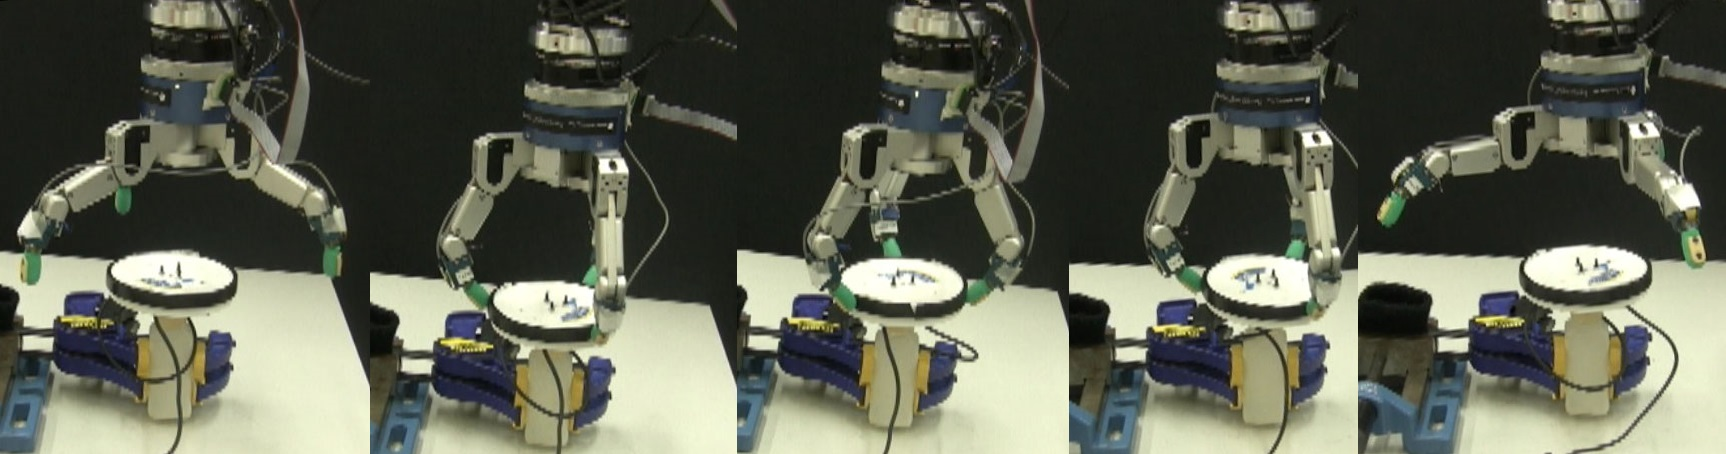
\includegraphics[width=13cm]{./fig_cha4/demo_b1.jpg}}

  \vspace{0.3cm}
  %\hspace{0.2cm}
  \subfloat[\scriptsize{Cap displacement during the robot's opening}]
  {
\includegraphics[width=13cm]{./fig_cha4/demo_b1_s.eps}}

  \vspace{0.3cm}
  \hspace{-0.3cm}
  \subfloat[\scriptsize{Torque exerted by the robot against cap displacement}]
  {
\includegraphics[width=13cm]{./fig_cha4/demo_b1_T.eps}}

  \vspace{0.3cm}
  %\vspace{0.5cm}
  \subfloat[\scriptsize{Responsibility factor against cap
    displacement, for each module}]
  {
\includegraphics[width=13cm]{./fig_cha4/demo_b1_rf.eps}}
  \caption{ \scriptsize{The robot opens bottle~$b1$.}
}

\label{fig:demo_b1}
\end{figure*}

\begin{figure*}
  \centering
  \vspace{0.8cm}
  \subfloat[\scriptsize{Snapshots from the robot opening bottle~$b4$}]
  {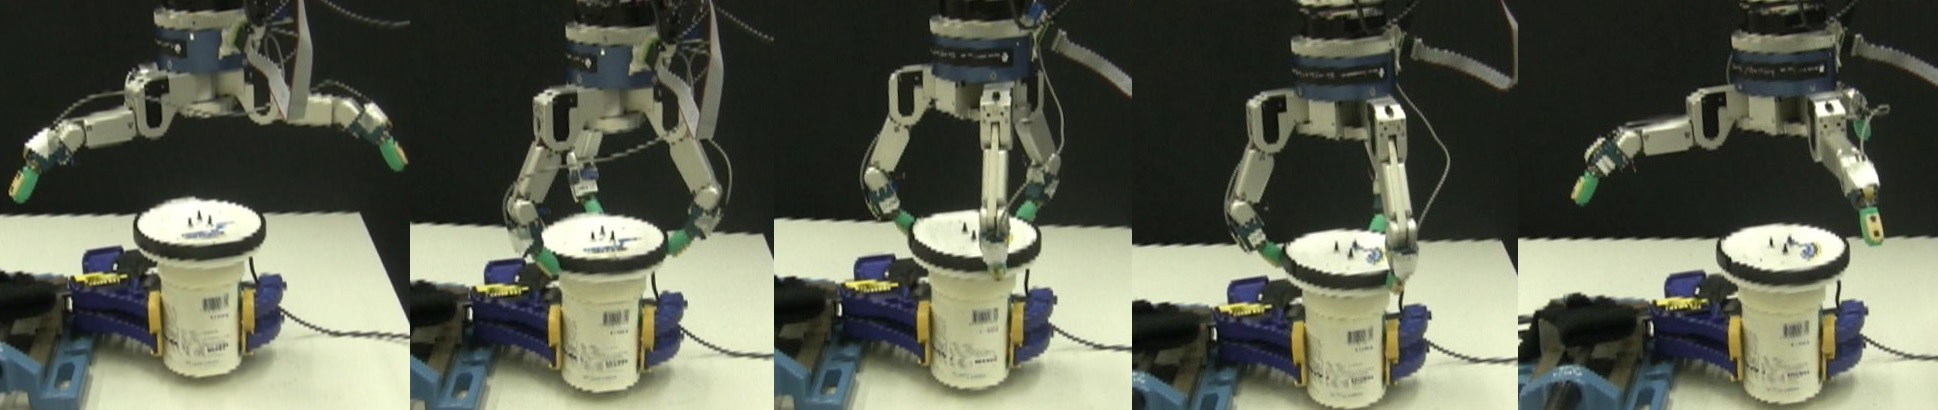
\includegraphics[width=13cm]{./fig_cha4/demo_b4.jpg}}

  \vspace{0.3cm}
  %\vspace{0.5cm}
  \subfloat[\scriptsize{Cap displacement during the robot's opening}]
  {
\includegraphics[width=13cm]{./fig_cha4/demo_b4_s.eps}}

  \vspace{0.3cm}
  \hspace{-0.2cm}
  \subfloat[\scriptsize{Torque exerted by the robot against cap displacement}]
  {
\includegraphics[width=13cm]{./fig_cha4/demo_b4_T.eps}}

  \vspace{0.3cm}
  %\vspace{0.5cm}
  \subfloat[\scriptsize{Responsibility factor against cap displacement, for each module}]
  {
\includegraphics[width=13cm]{./fig_cha4/demo_b4_rf.eps}}

  \caption{ \scriptsize{The robot opens bottle~$b4$}
}
\label{fig:demo_b4}
\end{figure*}

%JJB --- fix the captions for the below as I already did for the
%above. %JJB
\begin{figure*}
  \centering
  \vspace{0.8cm}
  \subfloat[\scriptsize{Snapshots for robot opening bottle~b5 demonstration}]
  {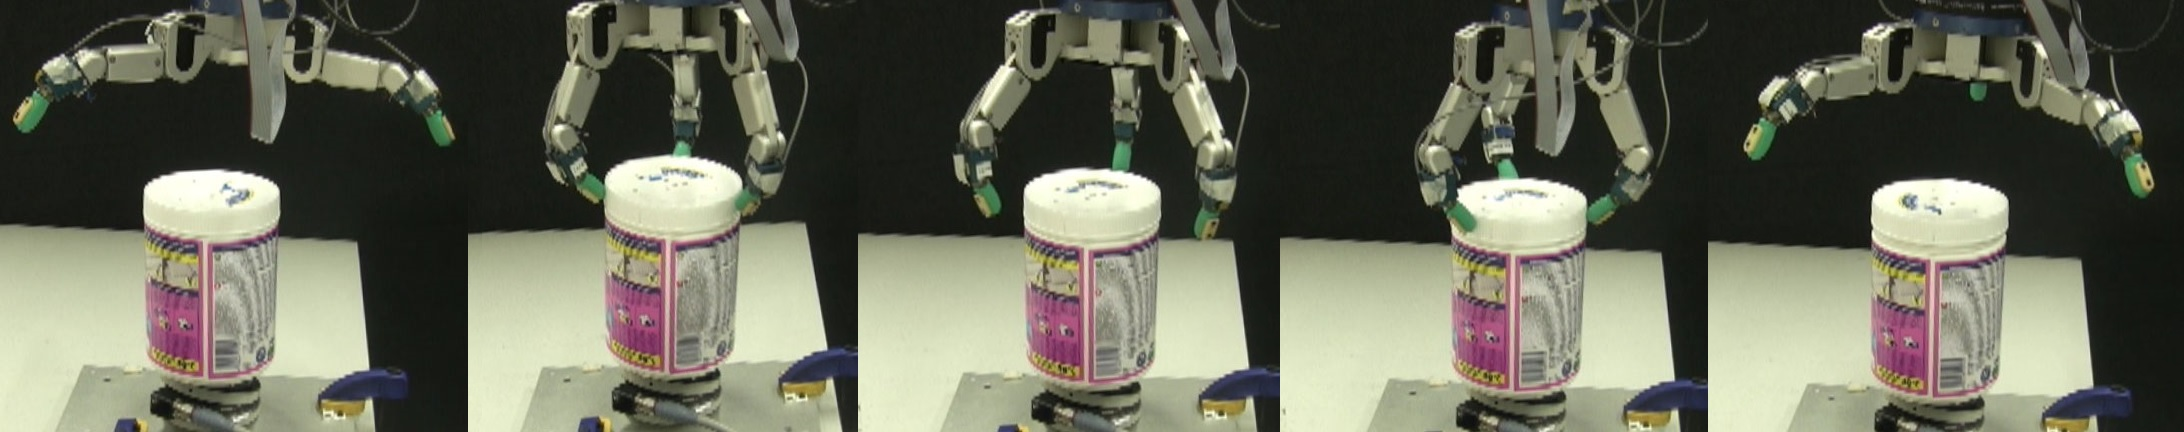
\includegraphics[width=13cm]{./fig_cha4/demo_b5.jpg}}

  \vspace{0.3cm}
  %\vspace{0.5cm}
  \subfloat[\scriptsize{Cap displacement during the robot's opening}]
  {
\includegraphics[width=13cm]{./fig_cha4/demo_b5_s.eps}}

  \vspace{0.3cm}
  %\vspace{0.5cm}
  \subfloat[\scriptsize{Torque exerted by the robot against cap displacement}]
  {
\includegraphics[width=13cm]{./fig_cha4/demo_b5_T.eps}}

  \vspace{0.3cm}
  %\vspace{0.5cm}
  \subfloat[\scriptsize{Responsibility factor against cap     displacement, for each module}]
  {
\includegraphics[width=13cm]{./fig_cha4/demo_b5_rf.eps}}

  \caption{ \scriptsize{The robot opens bottle~$b5$}
}
\vspace{5cm}
\label{fig:demo_b5}
\end{figure*}

\begin{figure*}
  \centering
  \vspace{0.8cm}
  \subfloat[\scriptsize{Snapshots for robot opening bottle~b6 demonstration}]
  {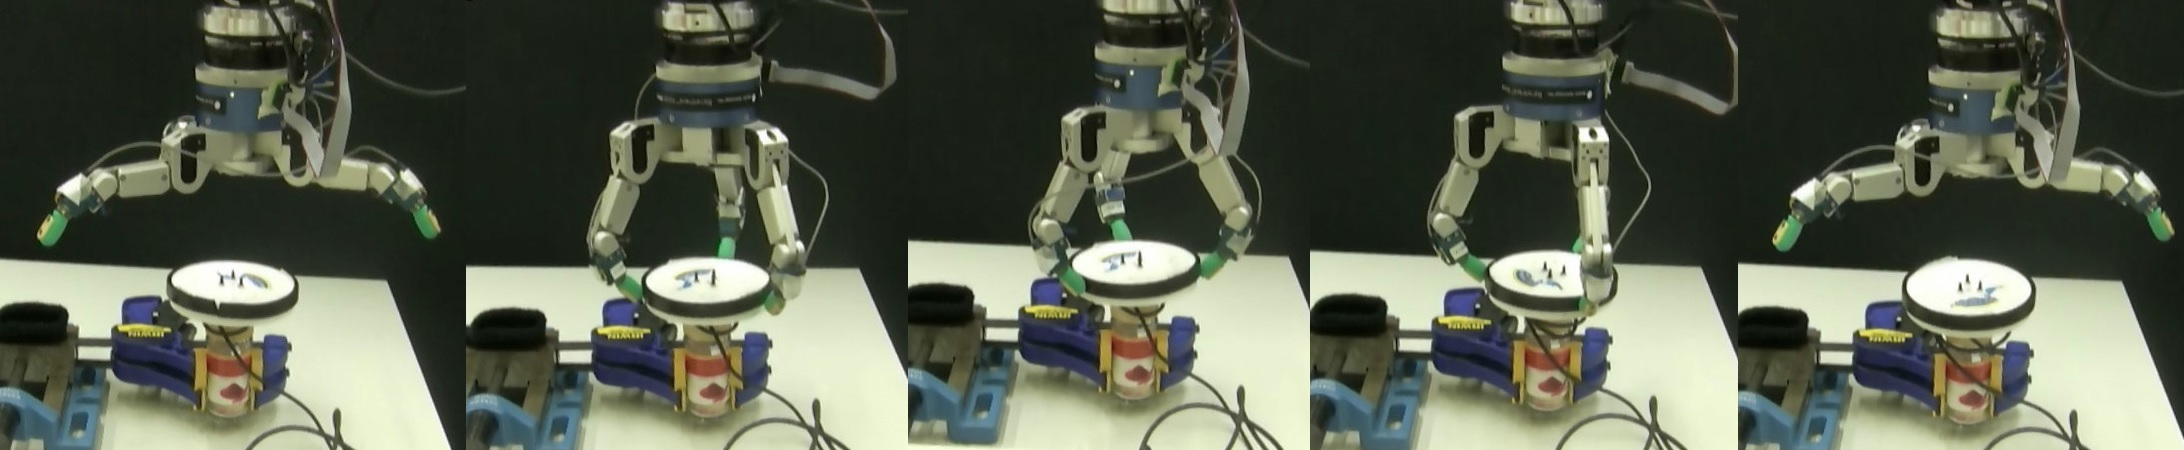
\includegraphics[width=13cm]{./fig_cha4/demo_b6.jpg}}

  \vspace{0.3cm}
  %\vspace{0.5cm}
  \subfloat[\scriptsize{Cap displacement during the robot's opening}]
  {
\includegraphics[width=13cm]{./fig_cha4/demo_b6_s.eps}}

  \vspace{0.3cm}
  \hspace{-0.5cm}
  \subfloat[\scriptsize{Torque exerted by the robot against cap displacement}]
  {
\includegraphics[width=13cm]{./fig_cha4/demo_b6_T.eps}}

  \vspace{0.3cm}
  %\vspace{0.5cm}
  \subfloat[\scriptsize{Responsibility factor against cap     displacement, for each module}]
  {
\includegraphics[width=13cm]{./fig_cha4/demo_b6_rf.eps}}

  \caption{ \scriptsize{The robot opens bottle~$b6$}
}
\label{fig:demo_b6}
\end{figure*}


\begin{figure}
  \centering
  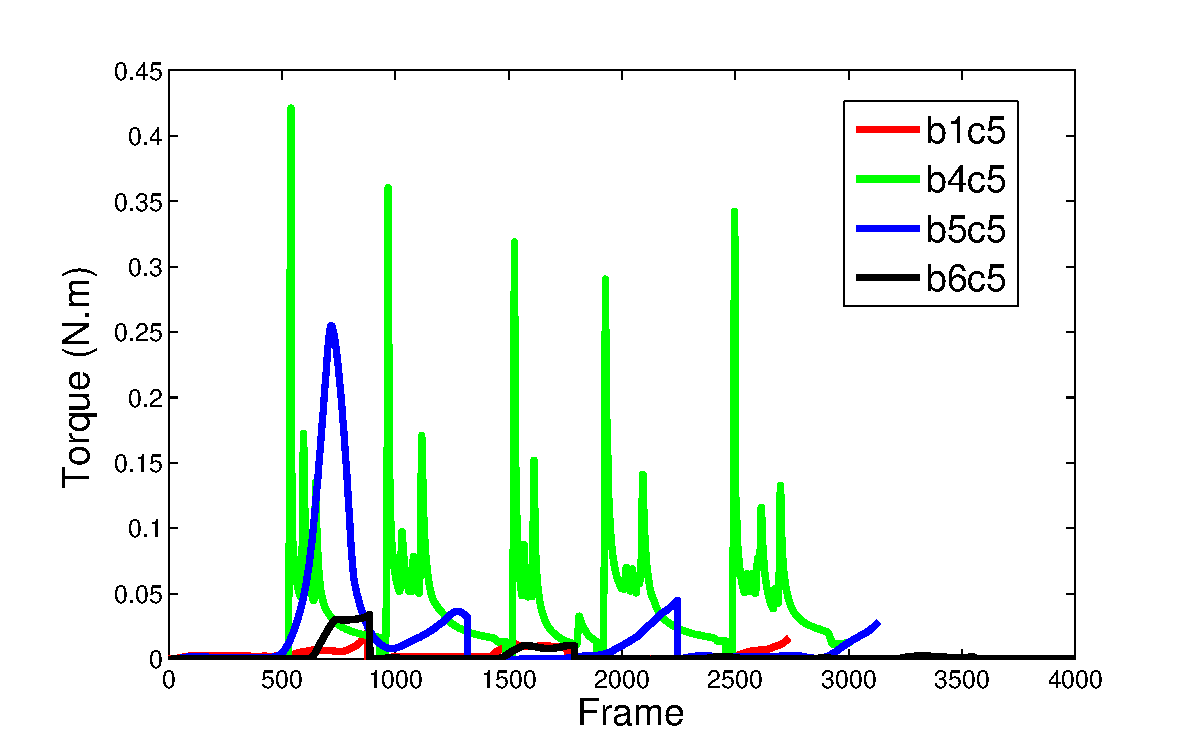
\includegraphics[width=8cm]{./fig_cha4/rb1b4b5b6_time_T.eps}
  \caption{ \scriptsize{Robot exerted torque for opening four bottles: b1 b4 b5 b6. Time is warped and shifted for displace purpose}
}
\label{fig:demo_b1b4b5b6}
\end{figure}



